%!TEX TS-program = xelatex

% Шаблон документа LaTeX создан в 2018 году
% Алексеем Подчезерцевым
% В качестве исходных использованы шаблоны
% 	Данилом Фёдоровых (danil@fedorovykh.ru) 
%		https://www.writelatex.com/coursera/latex/5.2.2
%	LaTeX-шаблон для русской кандидатской диссертации и её автореферата.
%		https://github.com/AndreyAkinshin/Russian-Phd-LaTeX-Dissertation-Template

\documentclass[a4paper,14pt]{article}


%%% Работа с русским языком
\usepackage[english,russian]{babel}   %% загружает пакет многоязыковой вёрстки
\usepackage{fontspec}      %% подготавливает загрузку шрифтов Open Type, True Type и др.
\defaultfontfeatures{Ligatures={TeX},Renderer=Basic}  %% свойства шрифтов по умолчанию
\setmainfont[Ligatures={TeX,Historic}]{Times New Roman} %% задаёт основной шрифт документа
\setsansfont{Comic Sans MS}                    %% задаёт шрифт без засечек
\setmonofont{Courier New}
%\usepackage{indentfirst}                      %% первый абзац с красной строки
\frenchspacing

\renewcommand{\epsilon}{\ensuremath{\varepsilon}}
\renewcommand{\phi}{\ensuremath{\varphi}}
\renewcommand{\kappa}{\ensuremath{\varkappa}}
\renewcommand{\le}{\ensuremath{\leqslant}}
\renewcommand{\leq}{\ensuremath{\leqslant}}
\renewcommand{\ge}{\ensuremath{\geqslant}}
\renewcommand{\geq}{\ensuremath{\geqslant}}
\renewcommand{\emptyset}{\varnothing}

%%% Дополнительная работа с математикой
\usepackage{amsmath,amsfonts,amssymb,amsthm,mathtools} % AMS
\usepackage{icomma} % "Умная" запятая: $0,2$ --- число, $0, 2$ --- перечисление

%% Номера формул
%\mathtoolsset{showonlyrefs=true} % Показывать номера только у тех формул, на которые есть \eqref{} в тексте.
%\usepackage{leqno} % Нумерация формул слева	

%% Перенос знаков в формулах (по Львовскому)
\newcommand*{\hm}[1]{#1\nobreak\discretionary{}
	{\hbox{$\mathsurround=0pt #1$}}{}}

%%% Работа с картинками
\usepackage{graphicx}  % Для вставки рисунков
\graphicspath{{images/}}  % папки с картинками
\setlength\fboxsep{3pt} % Отступ рамки \fbox{} от рисунка
\setlength\fboxrule{1pt} % Толщина линий рамки \fbox{}
\usepackage{wrapfig} % Обтекание рисунков текстом

%%% Работа с таблицами
\usepackage{array,tabularx,tabulary,booktabs} % Дополнительная работа с таблицами
\usepackage{longtable}  % Длинные таблицы
\usepackage{multirow} % Слияние строк в таблице
\usepackage{float}% http://ctan.org/pkg/float

%%% Программирование
\usepackage{etoolbox} % логические операторы


%%% Страница
\usepackage{extsizes} % Возможность сделать 14-й шрифт
\usepackage{geometry} % Простой способ задавать поля
\geometry{top=20mm}
\geometry{bottom=20mm}
\geometry{left=20mm}
\geometry{right=10mm}
%
%\usepackage{fancyhdr} % Колонтитулы
% 	\pagestyle{fancy}
%\renewcommand{\headrulewidth}{0pt}  % Толщина линейки, отчеркивающей верхний колонтитул
% 	\lfoot{Нижний левый}
% 	\rfoot{Нижний правый}
% 	\rhead{Верхний правый}
% 	\chead{Верхний в центре}
% 	\lhead{Верхний левый}
%	\cfoot{Нижний в центре} % По умолчанию здесь номер страницы

\usepackage{setspace} % Интерлиньяж
\onehalfspacing % Интерлиньяж 1.5
%\doublespacing % Интерлиньяж 2
%\singlespacing % Интерлиньяж 1

\usepackage{lastpage} % Узнать, сколько всего страниц в документе.

\usepackage{soul} % Модификаторы начертания

\usepackage{hyperref}
\usepackage[usenames,dvipsnames,svgnames,table,rgb]{xcolor}
\hypersetup{				% Гиперссылки
	unicode=true,           % русские буквы в раздела PDF
	pdftitle={Заголовок},   % Заголовок
	pdfauthor={Автор},      % Автор
	pdfsubject={Тема},      % Тема
	pdfcreator={Создатель}, % Создатель
	pdfproducer={Производитель}, % Производитель
	pdfkeywords={keyword1} {key2} {key3}, % Ключевые слова
	colorlinks=true,       	% false: ссылки в рамках; true: цветные ссылки
	linkcolor=black,          % внутренние ссылки
	citecolor=black,        % на библиографию
	filecolor=magenta,      % на файлы
	urlcolor=black           % на URL
}
\makeatletter 
\def\@biblabel#1{#1. } 
\makeatother
\usepackage{cite} % Работа с библиографией
%\usepackage[superscript]{cite} % Ссылки в верхних индексах
%\usepackage[nocompress]{cite} % 
\usepackage{csquotes} % Еще инструменты для ссылок

\usepackage{multicol} % Несколько колонок

\usepackage{tikz} % Работа с графикой
\usepackage{pgfplots}
\usepackage{pgfplotstable}

% ГОСТ заголовки
\usepackage[font=small]{caption}
%\captionsetup[table]{justification=centering, labelsep = newline} % Таблицы по правобу краю
%\captionsetup[figure]{justification=centering} % Картинки по центру


\usepackage{listings}
\newcommand{\listingsfont}{\small}
\lstset{
	%basicstyle=\small,
	basicstyle=\linespread{0.8}\listingsfont,
	numbers=left,
	breaklines=true,
	%backgroundcolor=\color{light-gray},
	tabsize=2,
	%basicstyle=\ttfamily,
	literate={\ \ }{{\ }}1
}

\newcommand{\tablecaption}[1]{\addtocounter{table}{1}\small \begin{flushright}\tablename \ \thetable\end{flushright}%	
\begin{center}#1\end{center}}

\newcommand{\imref}[1]{рис.~\ref{#1}}

\usepackage{multirow}
\usepackage{spreadtab}
\newcolumntype{K}[1]{@{}>{\centering\arraybackslash}p{#1cm}@{}}


\usepackage{xparse}
\ExplSyntaxOn
\DeclareExpandableDocumentCommand{\juliandate}{ m m m }
{
	\juliandate_calc:nnnn { #1 } { #2 } { #3 } { \use:n }
}
\NewDocumentCommand{\storejuliandate}{ s m m m m }
{
	\IfBooleanTF{#1}
	{
		\juliandate_calc:nnnn { #3 } { #4 } { #5 } { \cs_set:Npx #2 }
	}
	{
		\juliandate_calc:nnnn { #3 } { #4 } { #5 } { \cs_new:Npx #2 }
	}
}
\cs_new:Npn \juliandate_calc:nnnn #1 #2 #3 #4 % #1 = day, #2 = month, #3 = year, #4 = what to do
{
	#4 
	{
		\int_eval:n
		{
			#1 +
			\int_div_truncate:nn { 153 * (#2 + 12 * \int_div_truncate:nn { 14 - #2 } { 12 } - 3) + 2 } { 5 } +
			365 * (#3 + 4800 - \int_div_truncate:nn { 14 - #2 } { 12 } ) +
			\int_div_truncate:nn { #3 + 4800 - \int_div_truncate:nn { 14 - #2 } { 12 } } { 4 } -
			\int_div_truncate:nn { #3 + 4800 - \int_div_truncate:nn { 14 - #2 } { 12 } } { 100 } + 
			\int_div_truncate:nn { #3 + 4800 - \int_div_truncate:nn { 14 - #2 } { 12 } } { 400 } -
			32045
		}
	}
}

\tl_new:N \l__juliandate_g_tl
\tl_new:N \l__juliandate_dg_tl
\tl_new:N \l__juliandate_c_tl
\tl_new:N \l__juliandate_dc_tl
\tl_new:N \l__juliandate_b_tl
\tl_new:N \l__juliandate_db_tl
\tl_new:N \l__juliandate_a_tl
\tl_new:N \l__juliandate_da_tl
\tl_new:N \l__juliandate_y_tl
\tl_new:N \l__juliandate_m_tl
\tl_new:N \l__juliandate_d_tl
\int_new:N \l_juliandate_day_int
\int_new:N \l_juliandate_month_int
\int_new:N \l_juliandate_year_int

\cs_new:Npn \__juliandate_set:nn #1 #2
{
	\tl_set:cx { l__juliandate_#1_tl } { \int_eval:n { #2 } }
}
\cs_new:Npn \__juliandate_use:n #1
{
	\tl_use:c { l__juliandate_#1_tl }
}
\cs_new_protected:Npn \juliandate_reverse:n #1
{
	\__juliandate_set:nn { g }
	{ \int_div_truncate:nn { #1 + 32044 } { 146097 } }
	\__juliandate_set:nn { dg }
	{ \int_mod:nn { #1 + 32044 } { 146097 } }
	\__juliandate_set:nn { c }
	{ \int_div_truncate:nn { ( \int_div_truncate:nn { \__juliandate_use:n { dg } } { 36524 } + 1) * 3 } { 4 } }
	\__juliandate_set:nn { dc }
	{ \__juliandate_use:n { dg } - \__juliandate_use:n { c } * 36524 }
	\__juliandate_set:nn { b }
	{ \int_div_truncate:nn { \__juliandate_use:n { dc } } { 1461 } }
	\__juliandate_set:nn { db }
	{ \int_mod:nn { \__juliandate_use:n { dc } } { 1461 } }
	\__juliandate_set:nn { a }
	{ \int_div_truncate:nn { ( \int_div_truncate:nn { \__juliandate_use:n { db } } { 365 } + 1) * 3 } { 4 } }
	\__juliandate_set:nn { da }
	{ \__juliandate_use:n { db } - \__juliandate_use:n { a } * 365 }
	\__juliandate_set:nn { y }
	{
		\__juliandate_use:n { g } * 400 + 
		\__juliandate_use:n { c } * 100 + 
		\__juliandate_use:n { b } * 4 + 
		\__juliandate_use:n { a }
	}
	\__juliandate_set:nn { m }
	{ \int_div_truncate:nn { \__juliandate_use:n { da } * 5 + 308 } { 153 } - 2 }
	\__juliandate_set:nn { d }
	{ \__juliandate_use:n { da } - \int_div_truncate:nn { (\__juliandate_use:n { m } + 4) * 153 } { 5 } + 122 }
	\int_set:Nn \l_juliandate_year_int
	{ \__juliandate_use:n { y } - 4800 + \int_div_truncate:nn { \__juliandate_use:n { m } + 2 } { 12 } }
	\int_set:Nn \l_juliandate_month_int
	{ \int_mod:nn { \__juliandate_use:n { m } + 2 } { 12 } + 1 }
	\int_set:Nn \l_juliandate_day_int
	{ \__juliandate_use:n { d } + 1 }
}
\cs_generate_variant:Nn \juliandate_reverse:n { x }

\NewDocumentCommand{\showday}{ m }
{
	\juliandate_reverse:n { #1 }
	\int_to_arabic:n { \l_juliandate_day_int }-
	\int_to_arabic:n { \l_juliandate_month_int }-
	\int_to_arabic:n { \l_juliandate_year_int }
}

\NewDocumentCommand{\tomorrow}{ }
{
	\group_begin:
	\juliandate_reverse:x { \juliandate_calc:nnnn { \day + 1 } { \month } { \year } { \use:n } }
	\day = \l_juliandate_day_int
	\month = \l_juliandate_month_int
	\year = \l_juliandate_year_int
	\today
	\group_end:
}
\NewDocumentCommand{\tomorrowof}{ m m m }
{
	\group_begin:
	\juliandate_reverse:x { \juliandate_calc:nnnn { #1 + 1 } { #2 } { #3 } { \use:n } }
	\day = \l_juliandate_day_int
	\month = \l_juliandate_month_int
	\year = \l_juliandate_year_int
	\today
	\group_end:
}
\ExplSyntaxOff
\begin{document} % конец преамбулы, начало документа
\begin{titlepage}
	\begin{center}
		ФЕДЕРАЛЬНОЕ  ГОСУДАРСТВЕННОЕ АВТОНОМНОЕ \\
		ОБРАЗОВАТЕЛЬНОЕ УЧРЕЖДЕНИЕ ВЫСШЕГО ОБРАЗОВАНИЯ\\
		«НАЦИОНАЛЬНЫЙ ИССЛЕДОВАТЕЛЬСКИЙ УНИВЕРСИТЕТ\\
		«ВЫСШАЯ ШКОЛА ЭКОНОМИКИ»
	\end{center}
	
	\begin{center}
		\textbf{Департамент прикладной математики}
	\end{center}
	
	\vspace{12ex}
	
	\begin{center}
		\textbf{ОТЧЕТ\\
			К ЛАБОРАТОРНОЙ РАБОТЕ 4\\
			по дисциплине «Компьютерный практикум»
		}
	\end{center}
	
	\vspace{12ex}
	
	\begin{flushright}
		\begin{tabular}{lcr}
			Работу выполнила&&\\
			студентка группы БПМ 173 & $\underset{\text{дата, подпись}}{\underline{\hspace{4.5cm}}}$  & М.В. Самоделкина \\\\
			Работу проверил & $\underset{\text{дата, подпись}}{\underline{\hspace{4.5cm}}}$  &С.А. Булгаков \\\\
		\end{tabular}
	\end{flushright}
	
	\vfill
	
	\begin{center}
		Москва \the\year
	\end{center}
	
\end{titlepage}
\setcounter{page}{2} % нумерация

\renewcommand\contentsname{\centering {\normalsize Содержание}}
\tableofcontents
\newpage

\section*{Постановка задачи}
\addcontentsline{toc}{section}{Постановка задачи}

Реализовать загрузку растровых изображений и переработать функционал отрисовки объектов таким образом, чтобы для отображения объектов использовались изображения. Окончательно доработать логику игры.


\newpage

\section{Основная часть}
\subsection{Общая идея решения задачи}
В работе была реализована отрисовка объектов с помощью растровых изображений вместо геометрических фигур, используя класс \textit{QImage}. Была завершена разработка логики игры: появилась возможность отображать счет и количество жизней на экране, обработка столкновений пчелы и врагов. Был улучшен механизм взаимодействий объектов.

\subsection{Структура и принципы действия}
В классе конкретного посетителя \textit{DrawGameItems} был изменен механизм отрисовки объектов (функция \textit{visit}). С помощью класса \textit{QImage} и его методов \textit{load} и \textit{scaled} было загружено растровое изображение, которое масштабировалось под заданные размеры (в классе \textit{GameItem} появились поля \textit{sizeX} и \textit{sizeY} для хранения ширины и высоты объекта). Таким образом, объекты классов \textit{Bee}, \textit{Cloud}, \textit{Bell}, \textit{RedEnemy} и \textit{BlueEnemy} изображаются на экране с помощью выбранных картинок. Также был добавлен задний фон и установлены необходимые шрифты для отображения текста.

В классе \textit{Game} была улучшена функция \textit{Collide}, обрабатывающая столкновения объектов: стали использоваться поля \textit{sizeX} и \textit{sizeY} для расчета столкновений, была добавлена обработка взаимодействия врагов и пчелы; при их столкновении у пчелы отнимается жизнь, при этом количество жизней не может быть отрицательным? и потеря жизни не может происходить чаще заданного времени \textit{lifeTime}. Данный алгоритм описан в классе \textit{Bee} в функциях \textit{Update} и \textit{SubLifes}.

Был доработан механизм окончания игры: когда количество жизней достигает 0, то игра останавливается (перестает производиться обработка нажатий и отрисовка), выводится надпись \textit{"Game over"}.

\begin{figure}[H]
	\centering
	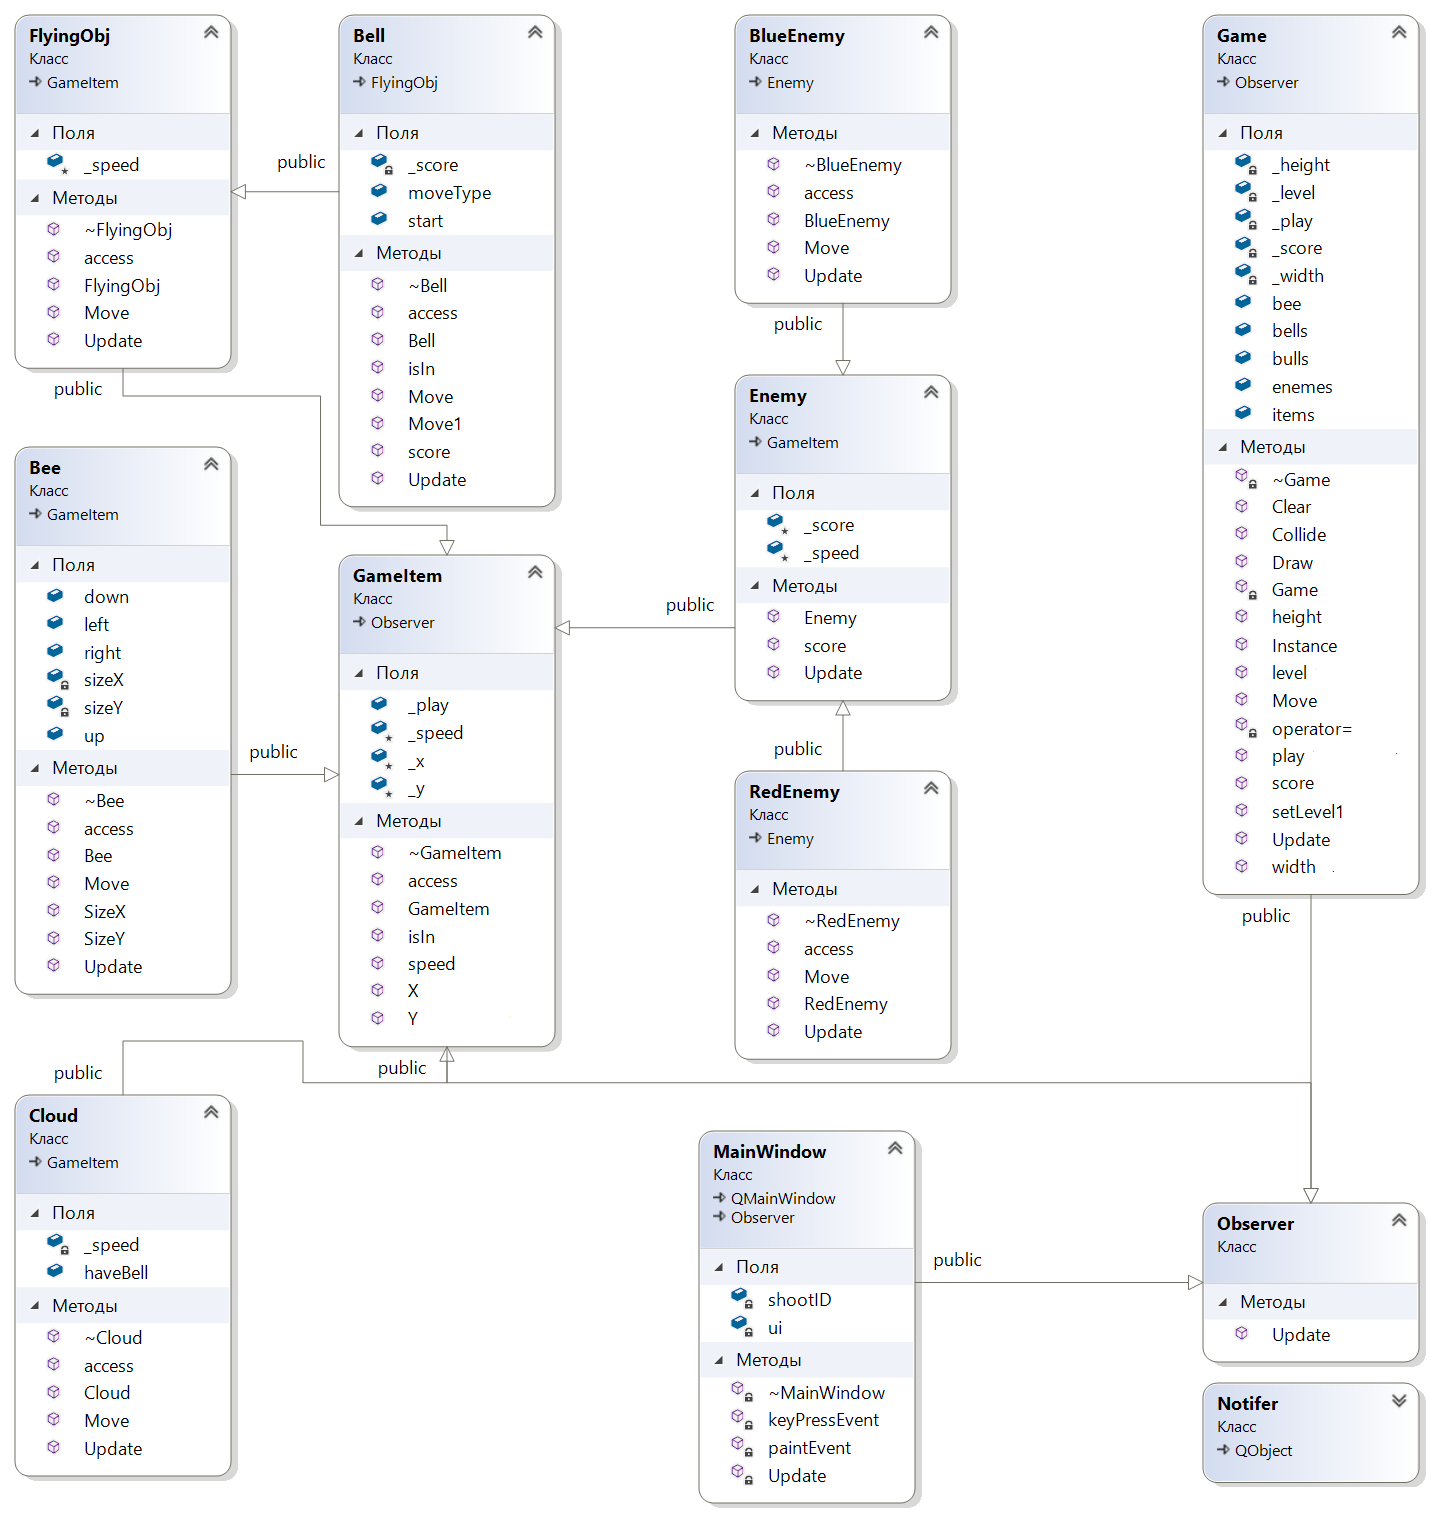
\includegraphics[width=\linewidth]{ClassDiagram1.png}
	\caption{Диграма классов}	
\end{figure}
\begin{figure}[H]
	\centering
	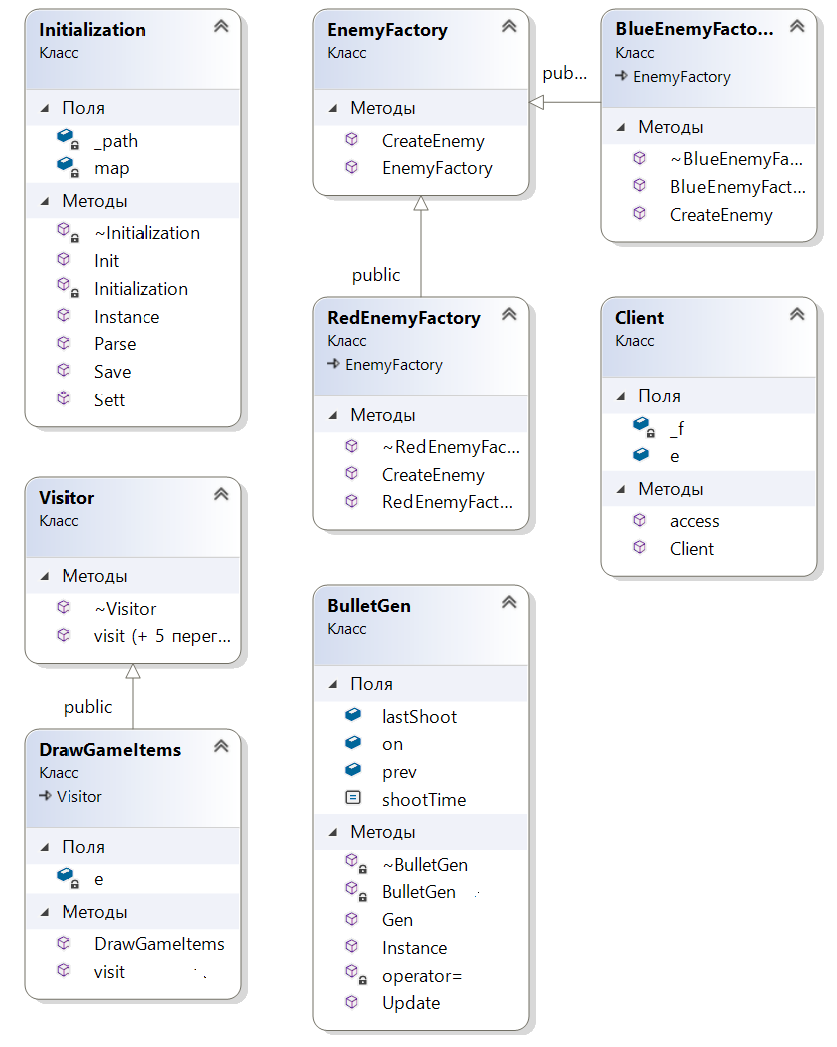
\includegraphics[width=\linewidth]{ClassDiagram2.png}
	\caption{Диграма классов (продолжение)}	
\end{figure}

\subsection{Процедура получения исполняемых программных модулей}
Программный код был скомпилирован с среде \textit{Qt Creator}. Компиляция раздельная: исходный код программы разделён на несколько файлов. Никаких дополнительных ключей не добавлялось, использовались ключи, которые добавляются по умолчанию. Параметры сборки: компилятор С++ MinGW 4.8.2, профиль Qt: Qt 4.8.7, отладчик GDB.
\subsection{Результаты тестирования}
Тестирование программы представлено в файле \textit{"main.cpp"} в функции \textit{Main()}. Ожидаемая отрисовка объектов в окне \textit{MainWindow}:

\begin{figure}[H]
	\centering
	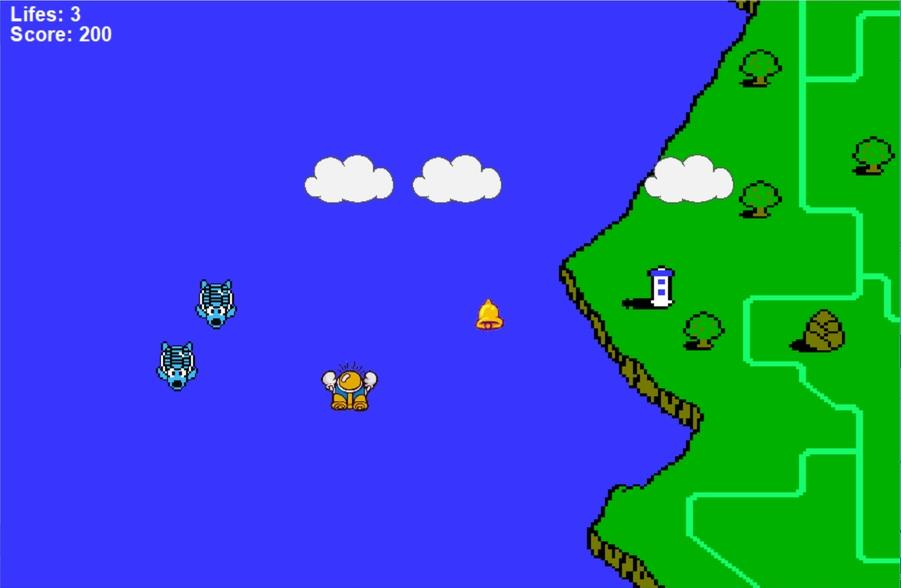
\includegraphics[width=\linewidth]{test.jpg}
	\caption{Результат тестирования}	
\end{figure}

\newpage
\setcounter{figure}{1} 
\setcounter{section}{1} 
\setcounter{subsection}{1} 

\begin{center}
	\section*{Приложение А}
	код программы (изменения)
	\addcontentsline{toc}{section}{Приложение А}
\end{center}
\renewcommand{\subsection}{\Asbuk{section}.\arabic{subsection}}
\setcounter{subsection}{1} 
\textbf{\subsection{  - MainWindow.cpp}}
\addcontentsline{toc}{subsection}{MainWindow.cpp}
\begin{lstlisting}
MainWindow::MainWindow(QWidget *parent) :
	QMainWindow(parent),
	ui(new Ui::MainWindow)
{
	ui->setupUi(this);
	Game& game = Game::Instance();
	this->setFixedSize(game.width(),game.height());
	Notifer::Instance().Subscribe(this);
	QPixmap bkgnd("images/back.png");
	bkgnd = bkgnd.scaled(this->size(), Qt::IgnoreAspectRatio);
	QPalette palette;
	palette.setBrush(QPalette::Background, bkgnd);
	this->setPalette(palette);
	QFont f( "Arial", 15, QFont::Bold);

	score = new QLabel(this);
	score->setFrameStyle(QFrame::Sunken);
	score->setGeometry(QRect(10,30,200,20));
	score->setStyleSheet("QLabel {color : white; }");
	score->setFont( f);
	lifes = new QLabel(this);
	lifes->setFrameStyle(QFrame::Sunken);
	lifes->setGeometry(QRect(10,10,200,20));
	lifes->setStyleSheet("QLabel {color : white; }");
	lifes->setFont( f);

	QFont f1( "Arial", 30, QFont::Bold);
	over = new QLabel(this);
	over->setFrameStyle(QFrame::Sunken);
	over->setGeometry(QRect(game.width()*0.36,game.height()/2,220,30));
	over->setStyleSheet("QLabel {color : white; }");
	over->setFont( f1);
};
\end{lstlisting}

\setcounter{subsection}{2} 
\textbf{\subsection{  - MainWindow.h}}
\addcontentsline{toc}{subsection}{MainWindow.h}
\lstinputlisting[language=C++]{versions/lab4/code/mainwindow.h}

\setcounter{subsection}{3} 
\textbf{\subsection{  - GameItem.cpp}}
\addcontentsline{toc}{subsection}{GameItem.cpp}
\lstinputlisting[language=C++]{versions/lab4/code/GameItem.cpp}

\setcounter{subsection}{4} 
\textbf{\subsection{  - Game.h}}
\addcontentsline{toc}{subsection}{Game.h}
\lstinputlisting[language=C++]{versions/lab4/code/Game.h}

\setcounter{subsection}{5} 
\textbf{\subsection{  - Bee.h}}
\addcontentsline{toc}{subsection}{Bee.h}
\lstinputlisting[language=C++]{versions/lab4/code/Bee.h}

\setcounter{subsection}{6} 
\textbf{\subsection{  - Bee.cpp}}
\addcontentsline{toc}{subsection}{Bee.cpp}
\lstinputlisting[language=C++]{versions/lab4/code/Bee.cpp}
\end{document} % конец документа
